\documentclass[brudnopis]{xmgr}
% Jeśli nowe rozdziały mają się zaczynać na stronach nieparzystych:
%\documentclass[openright]{xmgr}

% install minted package to highlight source code
% \usepackage{minted}

%\defaultfontfeatures{Scale=MatchLowercase}
%\setmainfont[Numbers=OldStyle,Ligatures=TeX]{Minion Pro}
%\setsansfont[Numbers=OldStyle,Ligatures=TeX]{Myriad Pro}
% for fontspec version < 2.0
% \setmainfont[Numbers=OldStyle,Mapping=tex-text]{Minion Pro}
% \setsansfont[Numbers=OldStyle,Mapping=tex-text]{Myriad Pro}
%\setmonofont[Scale=0.75]{Monaco}

% Opcjonalnie identyfikator dokumentu
% drukowany tylko z włączoną opcją 'brudnopis':
\wersja   {wersja wstępna [\ymdtoday]}

\author   {Adam Makiewicz}
\nralbumu {235281}
\email    {adammak23@gmail.com}


\title    {Generowanie płytek obwodu drukowanego w środowisku Python jako dodatek do programu graficznego Blender}
\date     {2020}
\miejsce  {Gdańsk}

\opiekun  {dr P. Arłukowicz}

% dodatkowe polecenia
%\renewcommand{\filename}[1]{\texttt{#1}}
%\definecolor{stress}{cmyk}{0,1,0.13,0} % RubineRed
%\definecolor{topic}{cmyk}{0.98,0.13,0,0.43} % MidnightBlue

\begin{document}

% streszczenie
\begin{abstract}
Istnieje wiele programów do projektowania płytek drukowanych, jednak żadne z nich, z uwagi na swoje ścisłe zastosowania, nie posiadają odpowiednich narzędzi do zaawansowanego renderowania, animacji i tworzenia szeroko pojętej “sztuki”. Popularny program do tworzenia grafiki 3D - Blender, z uwagi na możliwość rozbudowania go o dodatki jest znakomitym narzędziem mogącym wspomagać ten proces.
\end{abstract}

% słowa kluczowe
\keywords{wizualizacja, grafika, 3D, Blender, Python, PCB}

% tytuł i spis treści
\maketitle

% wstęp
\introduction

Obwody drukowane czy też inaczej płytki drukowane (zwane dalej "PCB", ang. Printed Circuit Board) to podstawa dla każdego modułu elektronicznego. Dzięki swojej budowie oraz dobranym częściom składowym pozwalają inżynierom z roku na rok konstruować coraz to nowocześniejsze i bardziej funkcjonalne urządzenia. PCB służy przede wszystkim do montowania wszelkich podzespołów elektronicznych oraz zapewnienia im wspólnego stabilnego połączenia.

Tworzenie PCB składa się z trzech głównych etapów \cite{Abboud}: 

\begin{itemize}
\item
Logic Design - Stworzenie schematu logiki i reguł projektowych, spis użytych komponentów i ich wzajemnych połączeń
\item
Layout - Zaprojektowanie układu, który decyduje o fizycznym położeniu i połączeniach (tzw.  \emph{routing}) komponentów
\item
Produkcja przemysłowa
\end{itemize}
    
    Najważniejszym punktem projektowania układu jest rozmieszczenie komponentów. Ten proces jest satysfakcjonującym twórczym przedsięwzięciem i prawdopodobnie jednym z najtrudniejszych aspektów procesu projektowania PCB. Wielu inżynierów uważa go za formę sztuki gdyż w przeciwieństwie do schematu, który opiera się tylko na matematyce, jest nieco bardziej płynny i elastyczny. 

\begin{figure}[!tbh]
\centering
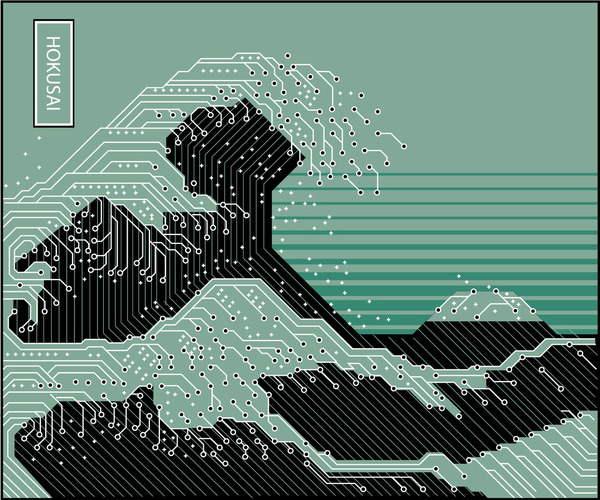
\includegraphics[width=1\hsize]{fig/hokusai}
\caption{Joel Betancourt znany jako Garabating - "Katsushika Hokusai Electronic Circuit Board"\label{RYS.1}}
\source{https://garabating.com/post/44549621917/katsushika-hokusai-electronic-circuit-board}
\end{figure}

Nie oznacza to jednak pełnej dowolności w projekcie, gdyż należy wziąć pod uwagę mnogość technicznej wiedzy, pomiarów i zależności takich jak optymalizacja długości ścieżek, ograniczenia mechaniczne i montażowe, itd.\footnote{https://www.autodesk.com/products/eagle/blog/top-10-pcb-component-placement-tips-pcb-beginner/} Z uwagi na ilość i różnorodność ograniczeń nie jest możliwa całkowita automatyzacja sprawdzania poprawności wykonanego projektu, zatem przydatna dla projektanta okazuje się wizualizacja efektu końcowego. Jest ona także niezbędnym elementem procesu marketingowego, logistycznego czy edukacyjnego. Istnieje wiele programów do projektowania PCB jednak żadne z nich, z uwagi na swoje ścisłe zastosowania, nie posiadają odpowiednich narzędzi do zaawansowanego renderowania, animacji i tworzenia szeroko pojętej “sztuki”. Popularny program do tworzenia grafiki 3D - Blender, z uwagi na możliwość rozbudowania go o dodatki jest znakomitym narzędziem mogącym wspomagać ten proces.


% ROZDZIAŁ 1


\chapter{Cel i zakres pracy magisterskiej}

Celem niniejszej pracy jest stworzenie łatwego do rozbudowania i spójnego systemu umożliwiającego import plików projektowych używanych bezpośrednio w przemyśle PCB do programu Blender, następnie interpretację i wyświetlenie pełnowymiarowego modelu 3D płytki drukowanej która powstałaby w procesie produkcji przemysłowej. Dodatek powinien posiadać prosty i przejrzysty interfejs który zapewnia dostęp do wszystkich funkcjonalności, ale nie przytłacza odbiorcy nadmiarem funkcji. Pozwoli to nie tylko osobom technicznym z poza branży grafiki komputerowej na łatwy dostęp do wizualizacji i edycji swoich projektów ale także na łatwiejszą integrację projektów przemysłowych z marketingową i graficzną częścią przemysłu.

\section{Wymagania funkcjonalne}

Zrealizowany system jest dodatkiem (tzw. \emph{add-on}) do programu Blender, kompatybilnym z wersją 2.8 w zwyż. Wybór konkretnie tej wersji programu był podyktowany jego nową odsłoną oferującą między innymi nowy interfejs i API. Addon udostępnia użytkownikowi dodatkowe funkcjonalności z poziomu graficznego interfejsu użytkownika:
\begin{itemize}
\item Wybranie folderu zawierającego wszystkie pliki projektu PCB lub wybranie pojedynczych plików warstw i  plików pozycji elementów (eng. \emph{"Pick And Place"})\footnote{Więcej o strukturze plików projektowych PCB w punkcie 1.2.3}
\item Wybranie wbudowanej lub własnej biblioteki modeli 3D
\item Wybór końcowej rozdzielczości i miejsca zapisu plików wytworzonych w procesie renderowania
\end{itemize}

\begin{figure}
\centering
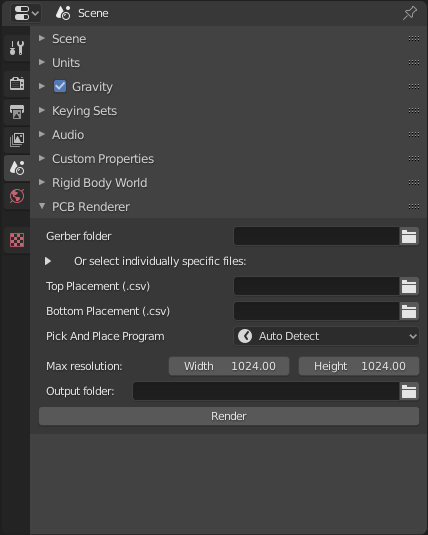
\includegraphics[width=0.75\hsize]{fig/addon_1}
\caption{Zainstalowany dodatek w programie Blender 2.82a\label{RYS.2}}
\source{Opracowanie własne}
\end{figure}

\section {Opis technologii wykorzystanych w pracy}

\subsection{Python}
Python jest językiem programowania wysokiego poziomu, posiadającym aktywną społeczność i nieograniczone możliwości poprzez rozbudowę go o zewnętrzne pakiety.\footnote {https://www.python.org/about/} API Blendera jest w większości przygotowane do użycia właśnie Pythona i chociaż istnieją ograniczenia tego, co Python może zrobić w Blenderze, jest to jedyne oficjalnie wspierane rozwiązanie dzięki któremu wiele można osiągnąć bez konieczności zagłębiania się w kod C / C++ Blendera.
\subsection {Blender 2.8}
Darmowy program \emph{Open-source}\footnote{https://www.blender.org/about/license/} cechujący się wszechstronnością i możliwością rozbudowania go o dodatkowe biblioteki lub skrypty napisane w języku Python, które poszerzają podstawowe funkcjonalności.

Dodatek do programu Blender różni się od dodatkowej biblioteki Pythona jedynie pewnymi dodatkowymi wymaganiami jak obiekt zawierający metadane, takie jak: tytuł, wersja, kategoria, autor, etc. Określa też minimalną wersję Blendera wymaganą do uruchomienia skryptu. Dodatek jest więc sposobem na enkapsulację modułu Pythona w sposób, który użytkownik może z łatwością wykorzystać.

Blender ma wbudowany interpreter Pythona, który jest ładowany po uruchomieniu programu. Utrudnia to znacząco wykorzystanie automatycznego pobierania i instalowania zależnych od siebie pakietów, co za tym idzie, tworzony w ramach pracy system, aby ułatwić korzystanie z niego, musi być niezależny od zewnętrznych, dynamicznie pobieranych bibliotek.

% może coś jeszcze tu wciśnąć


\subsection{opis plików projektowych PCB (gerber, excellon, placement, etc.)}
\subsection{developing w VS code? fajny linker kopiujący etc?}
\subsection{moduły zewnętrzne pythona: cairo, wheel, gerber etc.}


% ROZDZIAŁ 2

\chapter{Architektura zrealizowanego systemu/Implementacja}

\section {Koncepcyjna struktura projektu}
Może wrzucić to PO rozdziale 2? miałoby większy sens

\subsection{Założenia i wymagania projektowe}
\begin{itemize}
\item Czytanie, interpretacja plików excellon, gerber
\item renderowanie - cairo
\item renderowanie modelu z wymiarów warstwy outline
\item baza modeli do PickAndPlace (+tworzenie bazy modeli - importer *.wrl)
\end{itemize}
\subsection{Implementacja wzorca projektowego}
\begin{itemize}
\item omówienie MVVC
\item omówienie pokrótce plików projektu, podział na moduły - interfejs, logika, init (+ importer?)
\end{itemize}

\subsection{przegląd funkcjonalności}



\chapter{Szczegóły implementacyjne systemu}
\section{Podstawowe komponenty}
\section{Funkcjonalność panelu}

\chapter{Podsumowanie}

Aplikacja,  mimo  iż  jest  dedykowana  dla  projektów stworzonych w gEDA, KiCad,  jest  o  wiele  bardziej uniwersalna, ponieważ w praktyce wystarczy dodać modele, aby uzyskać format możliwy do odczytania. Podsumowując,  w  wyniku  prac  implementacyjnych  udało  się  zrealizować projekt,  który  jest  zgodny  z  przyjętymi  wcześniej  wymaganiami  i  założeniami przedstawionymi  na  etapie  opracowywania  koncepcji  rozwiązania.  Pomijając  jedną dużą modyfikację związaną ze zmianą metodologii postępowania, projekt powstałych klas pozostał w niezmienionej formie. Warto także zaznaczyć, że przyjęta architektura realizuje   wszystkie   postawione   wymagania   funkcjonalne.   Niestety   aplikacja   nie uniknęła wad. Jedną, ale za to dość poważną, jest spore zapotrzebowanie na pamięć przy przetwarzaniu dużych plików. Jednak dla mniejszych zbiorów danych wydajność czasowa jest na akceptowalnym poziomie. W  kolejnym  rozdziale  przedstawione  zostanie  podsumowanie całokształtu prac związanych z analizą oraz implementacją omawianej aplikacji.

\section{Realizacja założonych celów pracy magisterskiej}
\section {Problemy napotkane podczas realizacji systemu}
\section{Możliwości rozwoju systemu}
\section{Wnioski?}



\begin{table}[!htb]
\begin{tabular}{|l|l|l|} \hline
Nazwa & Autor      & Adres URL \\ \hline
\texttt{sablotron} & Ginger Alliance & \url{http://www.gingerall.com} \\ \hline
\texttt{Xt}        & J.~Clark & \url{http://www.jclark.com} \\ \hline
\texttt{4XSLT}     & FourThought & \url{http://www.fourthought.com} \\ \hline
\texttt{Saxon}     & Michael Kay &  \url{http://users.iclway.co.uk/mhkay/saxon} \\ \hline
\texttt{Xalan}     & Apache XML Project & \url{http://xml.apache.org} \\ \hline
\end{tabular}
\caption{Publicznie dostępne procesory XLST\label{zest:proces:xslt}}
\source{Opracowanie własne}
\end{table}


% zakończenie
\summary
Możliwości, jakie stoją przed archiwum prac magisterskich opartych na
XML-u, są ograniczone jedynie czasem, jaki należy poświęcić na pełną
implementację systemu. Nie ma przeszkód technologicznych do stworzenia
co najmniej równie doskonałego repozytorium, jak ma to miejsce w
przypadku ETD. Jeżeli chcemy w pełni uczestniczyć w rozwoju nowej ery
informacji, musimy szczególną uwagę przykładać do odpowiedniej
klasyfikacji i archiwizacji danych. Sądzę, że język XML znacznie to
upraszcza.

% załączniki (opcjonalnie):
%\appendix
%\chapter{Tytuł załącznika 1}
%Treść załącznika 1.


% literatura (obowiązkowo):
\bibliographystyle{unsrt}
\bibliography{literatura}

% spis tabel (jeżeli jest potrzebny):
\listoftables

% spis rysunków (jeżeli jest potrzebny):
\listoffigures

\oswiadczenie

\end{document}
